\begin{subsectionframemod}{Difference between Natural and Aerial Images}

    \only<1>{
        \begin{figure}
            \centering
            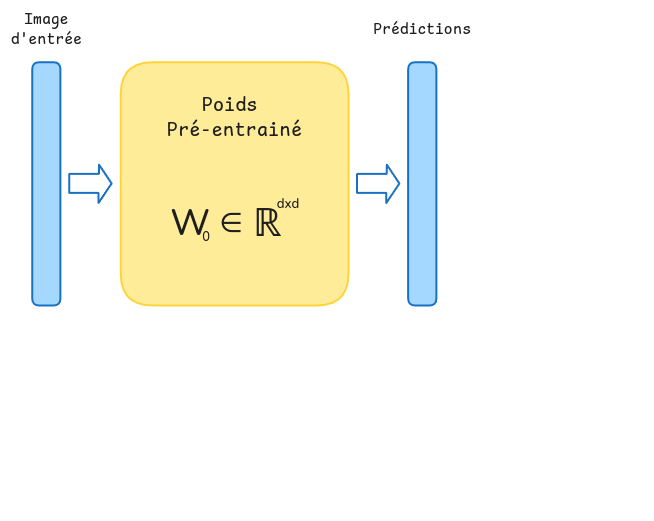
\includegraphics[width=0.6\textwidth]{Figures/lora_1}
            \caption{Schéma présentant LoRA (Low-Rank Adaptation), une technique permettant entre autre de limiter le risque d'overfitting pour assurer de meilleurs performances.}
        \end{figure}
    }
    \pause
    \only<2>{
        \begin{figure}
            \centering
            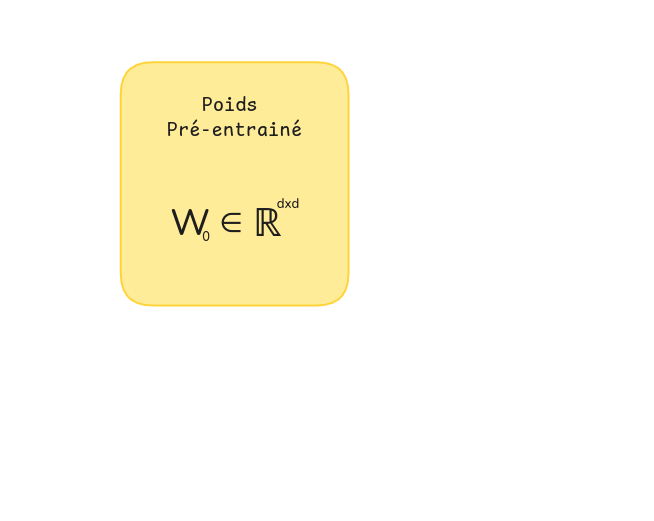
\includegraphics[width=0.6\textwidth]{Figures/lora_2}
            \caption{Schéma présentant LoRA (Low-Rank Adaptation), une technique permettant entre autre de limiter le risque d'overfitting pour assurer de meilleurs performances.}
        \end{figure}
    }
    \pause
    \only<3>{
        \begin{figure}
            \centering
            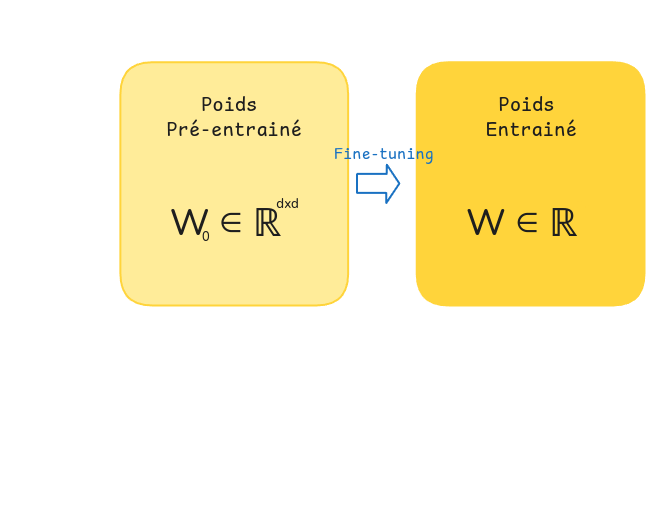
\includegraphics[width=0.6\textwidth]{Figures/lora_3}
            \caption{Schéma présentant LoRA (Low-Rank Adaptation), une technique permettant entre autre de limiter le risque d'overfitting pour assurer de meilleurs performances.}
        \end{figure}
    }
    \pause
    \only<4>{
        \begin{figure}
            \centering
            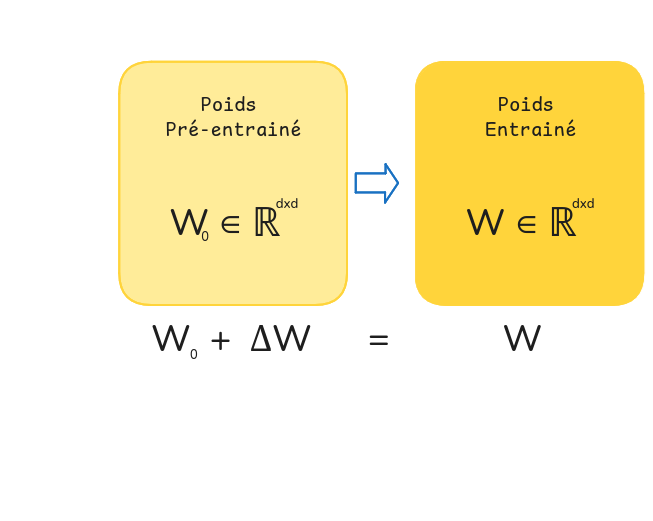
\includegraphics[width=0.6\textwidth]{Figures/lora_4}
            \caption{Schéma présentant LoRA (Low-Rank Adaptation), une technique permettant entre autre de limiter le risque d'overfitting pour assurer de meilleurs performances.}
        \end{figure}
    }
    \pause
    \only<5>{
        \begin{figure}
            \centering
            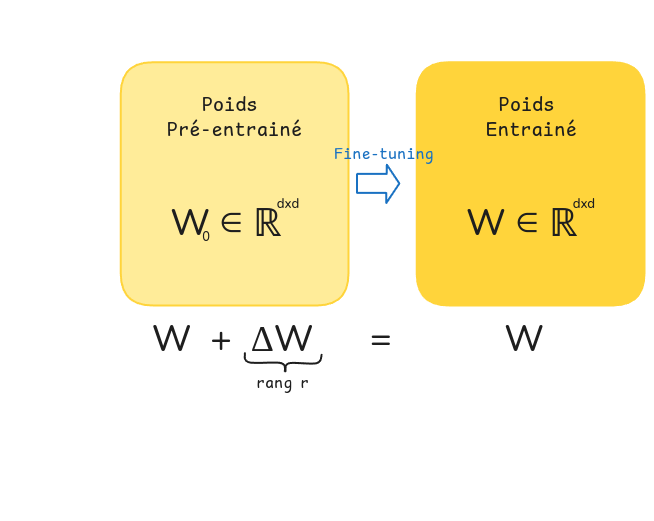
\includegraphics[width=0.6\textwidth]{Figures/lora_5}
            \caption{Schéma présentant LoRA (Low-Rank Adaptation), une technique permettant entre autre de limiter le risque d'overfitting pour assurer de meilleurs performances.}
        \end{figure}
    }
    \pause
    \only<6>{
        \begin{figure}
            \centering
            \includegraphics[width=0.6\textwidth]{Figures/lora_5-5}
            \caption{Schéma présentant LoRA (Low-Rank Adaptation), une technique permettant entre autre de limiter le risque d'overfitting pour assurer de meilleurs performances.}
        \end{figure}
    }
    \pause
    \only<7>{
        \begin{figure}
            \centering
            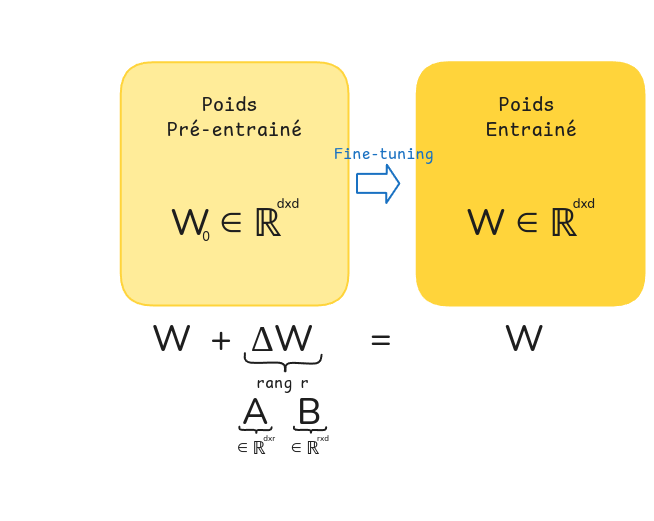
\includegraphics[width=0.6\textwidth]{Figures/lora_6}
            \caption{Schéma présentant LoRA (Low-Rank Adaptation), une technique permettant entre autre de limiter le risque d'overfitting pour assurer de meilleurs performances.}
        \end{figure}
    }


\end{subsectionframemod}